\section{The Laplace Transform}

While the methods used to solve second-order linear ODEs that were introduced in SVCDE and seen again in this course are useful, they can be awkward and time-consuming to apply in practice. The method involving the Laplace transform is useful more generally, and in particular in the cases where the ODE has impulsive forcing or discontinuous forcing. We shall introduce it now.

\subsection{Introduction}

\begin{definition}
	The Laplace transform $F(s)$ of $f(t)$ is
	\begin{equation}
		F(s) = \Lap{f}(s) = \int_0^{\infty} e^{-st}f(t)\,dt = \lim_{T \to \infty} \int_0^T e^{-st}f(t)\,dt.
	\end{equation}
\end{definition}

\begin{eg}\label{eg:laplacetrans}\hfill
	\begin{itemize}
		\item For $f(t)=1$,
		\[
			F(s) = \int_0^{\infty} e^{-st}\,dt = \left[\frac{e^{-st}}{-s}\right]_0^{\infty} = \frac{1}{s}. \tag{$s>0$}
		\]
		\item For $f(t)=e^{at}$,
		\[
			F(s) = \int_0^{\infty} e^{-st}e^{at}\,dt = \left[\frac{e^{-(s-a)t}}{-(s-a)}\right]_0^{\infty} = \frac{1}{s-a}. \tag{$s>a$}
		\]
		\item For $f(t) = \sin(at)$,
		\begin{align*}
			F(s) &= \int_0^{\infty} e^{-st}\sin(at) \,dt \\
			&= \left[e^{-st}\frac{\cos(at)}{a}\right]_0^{\infty} - \frac{s}{a}\int_0^{\infty} e^{-st}\cos(at) \,dt \\
			&= \frac{1}{a} - \frac{s}{a}\int_0^{\infty} e^{-st}\cos(at) \,dt \\
			&= \frac{1}{a} - \frac{s^2}{a^2}\int_0^{\infty} e^{-st}\sin(at) \,dt \\
			\left(1+\frac{s^2}{a^2}\right) F(s) &= \frac{1}{a} \\
			F(s) &= \frac{a}{s^2+a^2}. \tag{$s>0$}
		\end{align*}
		\item For $f(t) = \cos(at)$,
		\[
			F(s) = \frac{s}{s^2+a^2}.
		\]
		
	\end{itemize}
\end{eg}

Another way of writing the above results is that $\Lap{e^{at}} = \frac{1}{s-a}$, etc.

\begin{theorem}
	The Laplace transform of $f(t)$ exists for $s$ large enough provided that
	\begin{itemize}
		\item $f(t)$ is piecewise continuous,
		\item $|f(t)| \leq Ae^{Bt}$.
	\end{itemize}
\end{theorem}

In this theorem, the first condition is necessary for the integral $\int_0^{\infty} e^{-st}f(t)\,dt$ to exist. The second condition is necessary to bound $F(s)$:
\[
|F(s)| \leq \int_0^{\infty} e^{-st}|f(t)|\,dt \leq A\int_0^{\infty} e^{-st}e^{Bt}\,dt < \infty \quad\text{if } s>B.
\]

Key Properties of the Laplace transform:
\begin{enumerate}
	\item Linearity: $\Lap{c_1f_1(t) + c_2f_2(t)} = c_1\Lap{f_1} + c_2\Lap{f_2}$.
	\item $\Lap{f'} = s\Lap{f} - f(0)$.
\end{enumerate}

\begin{proof}\hfill
	\begin{enumerate}
		\item Follows easily from the linearity of the integral.
		\item Assuming the Laplace transform $\Lap{f}$ is well-defined,
		\begin{align*}
			\Lap{f'} = \int_0^{\infty} e^{-st}f'(t)\,dt &= \left[e^{-st}f(t)\right]_0^{\infty} + s\int_0^{\infty} e^{-st}f(t)\,dt \\
			&= s\Lap{f} - f(0).
		\end{align*}
	\end{enumerate}
\end{proof}

The Laplace transform for higher derivatives may be computed using the equation for $\Lap{f'}$:
\begin{align*}
	\Lap{f^{(n)}} &= s\Lap{f^{(n-1)}} - f^{(n-1)}(0) \\
	&= s^2\Lap{f^{(n-2)}} - sf^{(n-2)}(0) - f^{(n-1)}(0) \\
	&= s^n\Lap{f} - s^{n-1}f(0) - s^{n-2}f'(0) - \cdots - f^{(n-1)}(0).
\end{align*}

\subsection{Solving ODEs}

The method of using the Laplace transform to solve second-order linear ODEs is best illustrated with an example.

\begin{eg}
	We solve the ODE
	\[
	y''-y'-2y = 0 \quad\text{with}\quad y(0)=1, \,\,y'(0)=0.
	\]
	We apply the Laplace transform to the whole equation, writing $Y(s) = \Lap{y}$ and using the initial conditions to simplify:
	\begin{align*}
		s^2Y(s) - s\cancelto{1}{y(0)} - \cancelto{0}{y'(0)} - sY(s) + \cancelto{1}{y(0)} - 2Y(s) &= 0 \\
		(s^2-s-2)Y(s) &= s-1 \\
		Y(s) &= \frac{s-1}{s^2-s-2}.
	\end{align*}
	Now that we know $Y(s)$, what we really want is a formula to invert the Laplace transform and recover $y(t)$. In fact, such a formula exists:
	\[
	y(t) = \frac{1}{2\pi i} \int_{\gamma-i\infty}^{\gamma+i\infty} e^{st}Y(s) \,ds.
	\]
	However, this formula is quite complicated to apply, as it involves integrating along the line $\Re(s) = \gamma$ in the complex plane. Therefore, we shall generally invert the Laplace transform by inspection.
	
	Recall from \Cref{eg:laplacetrans} that $\Lap{e^{at}} = \frac{1}{s-a}$. We can write $Y(s)$ in this form by using partial fractions:
	\begin{align*}
		Y(s) = \frac{s-1}{s^2-s-2} &= \frac{A}{s-2} + \frac{B}{s+1} \\
		&= \frac13\cdot\frac{1}{s-2} + \frac23\cdot\frac{1}{s+1} \\
		&= \frac13\Lap{e^{2t}} + \frac23\Lap{e^{-t}} \\
		\implies y(t) &= \frac13e^{2t} + \frac23e^{-t}.
	\end{align*}
	This can easily be checked by applying the methods we know from before of finding the characteristic equation, getting exponential solutions, applying the initial conditions, and so on.
\end{eg}

\begin{eg}
	We solve the ODE
	\[
	y''+y = \sin(2t) \quad\text{with}\quad y(0)=2, \,\,y'(0)=1.
	\]
	Applying the Laplace transform and using the initial conditions:
	\begin{align*}
		s^2Y - 2s - 1 + Y &= \frac{2}{s^2+4} \\
		(s^2+1)Y &= \frac{2}{s^2+4} +2s+1 \\
		(s^2+1)Y &= \frac{2s^3+s^2+8s+6}{s^2+4} \\
		Y(s) &= \frac{2s^3+s^2+8s+6}{(s^2+1)(s^2+4)}.
	\end{align*}
	We wish to write $Y(s)$ as its partial fraction decomposition:
	\begin{align*}
		Y(s) = \frac{2s^3+s^2+8s+6}{(s^2+1)(s^2+4)} &= \frac{As+B}{s^2+1} + \frac{Cs+D}{s^2+4} \\
		2s^3+s^2+8s+6 &= (As+B)(s^2+4) + (Cs+D)(s^2+1).
	\end{align*}
	Equating coefficients gives the following system of equations:
	\begin{equation*}
		\begin{alignedat}{2}
			&s^3 &&: 2 = A+C \\
			&s^2 &&: 1 = B+D \\
			&s &&: 8 = 4A+C \\
			&s^0 &&: 6 = 4B+D.
		\end{alignedat}
	\end{equation*}
	Subtracting the first equation from the third yields
	\[
	3A = 6 \implies A = 2 \implies C=0,
	\]
	and subtracting the second equation from the fourth gives
	\[
	3B = 5 \implies B = \frac53 \implies D = -\frac23.
	\]
	Therefore
	\begin{align*}
		Y(s) &= \frac{2s}{s^2+1} + \frac53\cdot\frac{1}{s^2+1} - \frac13\cdot\frac{2}{s^2+4} \\
		&= 2\Lap{\cos{t}} + \frac53\Lap{\sin{t}} - \frac13\Lap{\sin(2t)} \\
		\implies y(t) &= 2\cos{t} + \frac53\sin{t} - \frac13\sin(2t).
	\end{align*}
\end{eg}

\subsection{Calculating the Laplace Transform for More Functions}

Now that we've seen how to use the Laplace transform to solve ODE, we see that it's important to have a `dictionary' of functions $f(t)$ and their transform $F(s)$. In that vein, we build on the few transforms found in \Cref{eg:laplacetrans}.

More properties of the Laplace transform:
\begin{enumerate}
	\item s-shift: $\Lap{e^{-ct}f(t)} = F(s+c)$.
	\item t-shift: $\Lap{f(t-c)} = e^{-sc}F(s)$ if $c \geq 0$ and $f(t)=0$ for $t<0$.
	\item Derivative in $s$: $\Lap{tf(t)} = -\frac{d}{ds}F(s)$.
	\item Scaling: $\Lap{f(ct)} = \frac{1}{c} F\left(\frac{s}{c}\right)$.
\end{enumerate}

\begin{proof}\hfill
	All three properties essentially follow from the definition of the Laplace transform.
	\begin{enumerate}
		\item \[\Lap{e^{-ct}f(t)} = \int_0^{\infty} e^{-st}e^{-ct}f(t) \,dt = \int_0^{\infty} e^{-(s+c)t}f(t) \,dt = F(s+c).\]
		\item Let $u=t-c$, then
		\[
			\int_0^{\infty} e^{-st}f(t-c) \,dt = \int_{-c}^{\infty} e^{-s(u+c)}f(u) \,du = \int_0^{\infty} e^{-sc}e^{-su}f(u) \,du = e^{-sc}F(s).
		\]
		\item \[\Lap{tf(t)} = \int_0^{\infty} e^{-st}tf(t) \,dt = \int_0^{\infty} -\frac{d}{ds}\left(e^{-st}\right) f(t) \,dt = -\frac{d}{ds} \int_0^{\infty} e^{-st}f(t) \,dt = -\frac{d}{ds}F(s).\]
		\item We have
		\[
		\Lap{f(ct)} = \int_0^{\infty} e^{-st}f(ct)\,dt = \int_0^{\infty} e^{-(s/c)ct}f(ct)\,dt.
		\]
		Making a change of variables $u=ct$ (with $dt = \frac{1}{c}du$) yields
		\[
		\Lap{f(ct)} = \int_0^{\infty} e^{-(s/c)ct}f(ct)\,dt = \frac{1}{c} \int_0^{\infty} e^{-(s/c)u}f(u)\,du = \frac{1}{c} F\left(\frac{s}{c}\right).
		\]
	\end{enumerate}
\end{proof}

\begin{eg}
	Using these properties, we calculate the Laplace transform for a few more functions.
	\begin{itemize}
		\item First, using the s-derivative property,
		\[
		\Lap{t} = \Lap{t\cdot 1} = -\frac{d}{ds}\Lap{1} = -\frac{d}{ds} \frac{1}{s} = \frac{1}{s^2}.
		\]
		\item By repeated application of the s-derivative,
		\[
		\Lap{t^n} = \frac{n!}{s^{n+1}}.
		\]
		\item Also using the s-derivative,
		\[
		\Lap{te^{at}} = -\frac{d}{ds} \Lap{e^{at}} = -\frac{d}{ds} \frac{1}{s-a} = \frac{1}{(s-a)^2}.
		\]
		\item Applying the s-shift property to $\Lap{\cos(at)} = \frac{s}{s^2+a^2}$,
		\[
		\Lap{e^{bt}\cos(at)} = \frac{s-b}{(s-b)^2+a^2}.
		\]
		\item Similarly, applying the s-shift to $\Lap{\sin(at)} = \frac{a}{s^2+a^2}$ gives,
		\[
		\Lap{e^{bt}\sin(at)} = \frac{a}{(s-b)^2+a^2}.
		\]
		\item By repeated application of the s-derivative, we can find that
		\[
		\Lap{t^nf(t)} = (-1)^n \frac{d}{ds}F(s).
		\]
		\item Using the previous result, we find
		\[
		\Lap{t^ne^{bt}\cos(at)} = (-1)^n\frac{d}{ds} \left(\frac{s-b}{(s-b)^2+a^2}\right),
		\]
		and a similar relation for $\Lap{t^ne^{bt}\sin(at)}$:
		\[
		\Lap{t^ne^{bt}\sin(at)} = (-1)^n\frac{d}{ds} \left(\frac{a}{(s-b)^2+a^2}\right).
		\]
	\end{itemize}
\end{eg}

Overall, what this example tells us is that when we apply the Laplace transform to functions of the form $g(t) = t^ne^{bt}\cos(at)$ and $h(t) = t^ne^{bt}\sin(at)$ (i.e. those that are a product of a power, exponential, and trigonometric function) the result is a rational function. These functions $g$ and $h$ are precisely the types of functions that appear as the RHS in ODEs we have solved previously using, for example, the method of undetermined coefficients. Thus, it is very helpful that we can get back to them by inverting the Laplace transform from a rational function.

\begin{remark}
	It is also possible to find $\Lap{e^{at}}$ using the s-shift property applied to $\Lap{1} = \frac{1}{s}$.
\end{remark}

For reference, a table of elementary Laplace transforms is given in \Cref{table:laplace} in \Cref{sec:laptable}.

\begin{eg}
	We solve the ODE
	\[
	y''-2y'+2y=2e^t \quad\text{with}\quad y(0)=0, \,\,y'(0)=1.
	\]
	Applying the Laplace transform:
	\begin{align*}
		s^2Y(s) - s\cancelto{0}{y(0)} - \cancelto{1}{y'(0)} - 2sY(s) + 2\cancelto{0}{y(0)} + 2Y(s) &= \frac{2}{s-1} \\
		s^2Y(s) - 1 - 2sY(s) + 2Y(s) &= \frac{2}{s-1} \\
		(s^2-2s+2)Y(s) &= \frac{2}{s-1} + 1 \\
		(s^2-2s+2)Y(s) &= \frac{s+1}{s-1} \\
		Y(s) &= \frac{s+1}{(s-1)(s^2-2s+2)}.
	\end{align*}
	As before, we write $Y(s)$ in terms of partial fractions:
	\begin{align*}
		Y(s) = \frac{s+1}{(s-1)(s^2-2s+2)} &= \frac{A}{s-1} + \frac{Bs+C}{(s-1)^2+1} \\
		s+1 &= A((s-1)^2+1) + (Bs+C)(s-1).
	\end{align*}
	Choosing $s=1$ tells us that $A=2$. For finding $B$ and $C$, we equate coefficients:
	\begin{align*}
		&s^2 : 0 = A+B \implies B=-2 \\
		&s^0 : 1 = 2A-C \implies C=3.
	\end{align*}
	Hence
	\begin{align*}
		Y(s) &= \frac{2}{s-1} - \frac{2s-3}{(s-1)^2+1} \\
		&= \frac{2}{s-1} - \frac{2(s-1)-1}{(s-1)^2+1} \\
		&= \frac{2}{s-1} - 2\frac{s-1}{(s-1)^2+1} + \frac{1}{(s-1)^2+1} \\
		&= 2\Lap{e^t} - 2\Lap{e^t\cos{t}} + \Lap{e^t\sin{t}} \\
		\implies y(t) &= 2e^t - 2e^t\cos{t} + e^t\sin{t}.
	\end{align*}
\end{eg}

\subsection{Solving ODEs with Discontinuous Forcing}

The Laplace transform is particularly efficient in solving ODEs where the RHS is a discontinuous function.

To work with such ODEs, we first introduce the \vb{unit step function} (also known as the Heaviside function):
\begin{equation}
	u_c(t) = \begin{cases}0 & \text{if } t<c \\ 1 & \text{if } t \geq c\end{cases}.
\end{equation}
This function is useful when we want to `clip' a function $f(t)$, i.e. only take the part of the function between $a$ and $b$:
\[
f_{\text{clip}}(t) = f(t)\left(u_a(t) - u_b(t)\right),
\]
or shift the function so that it is zero for all $t \leq c$:
\[
f_{\text{shift}} = f(t-c)u_c(t).
\]

\begin{figure}[!ht]
	\centering
	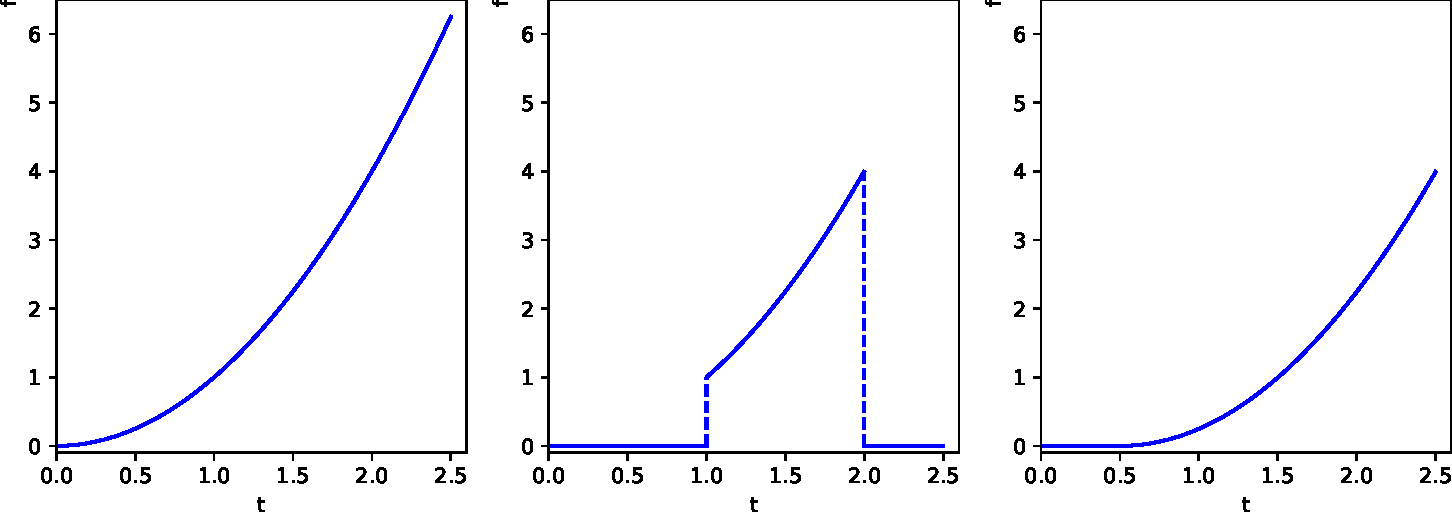
\includegraphics[width=0.9\textwidth]{ClippedFunctions.pdf}
	\caption{The function $f(x)=x^2$ (left), the `clipped' function with $a=1$ and $b=2$ (centre), and the `shifted' function with $c=\frac12$ (right).}
	\label{fig:clipping}
\end{figure}

The Laplace transform of the unit step function ($c \geq 0$) is
\[
	\Lap{u_c(t)} = \int_0^{\infty} e^{-st}u_c(t)\,dt = \int_c^{\infty}e^{-st}\,dt = \frac{e^{-sc}}{s}, \quad s>0.
\]
Here we can see a connection to the t-shift property of the Laplace transform from earlier, which stated that $\Lap{f(t-c)} = e^{-sc}F(s)$ if $c \geq 0$ and $f(t)=0$ for $t<0$. Functions satisfying these conditions can be nicely described as $f(t-c)u_c(t)$, thus
\begin{equation}\label{eq:laplacediscont}
	\Lap{f(t-c)u_c(t)} = e^{-sc}F(s).
\end{equation}

This property can also be proved more directly:
\begin{proof}
	From the definition of the Laplace transform,
	\[
	\Lap{f(t-c)u_c(t)} = \int_0^{\infty} e^{-st}f(t-c)u_c(t) \,dt.
	\]
	Applying the change of variables $t-c=t'$,
	\begin{align*}
		\int_0^{\infty} e^{-st}f(t-c)u_c(t) \,dt &= \int_{-c}^{\infty} e^{-s(t'+c)}f(t') \underbrace{u_c(t'+c)}_{=u_0(t')} \,dt' \\
		&= e^{-sc} \int_0^{\infty} e^{-st'}f(t') \,dt' \\
		&= e^{-sc} F(s).
	\end{align*}
\end{proof}

\begin{eg}
	Find the inverse Laplace transform of 
	\[
	F(s) = \frac{1-e^{-2s}}{s^2}.
	\]
	We will make use of the above property, and the fact that $\Lapinv{\frac{1}{s^2}} = t$.
	\begin{align*}
		f(t) &= \Lapinvb{\frac{1}{s^2}} - \Lapinvb{\frac{e^{-2s}}{s^2}} \\
		&= t - (t-2)u_2(t).
	\end{align*}
\end{eg}

Now we solve an ODE with discontinuous RHS:

\begin{eg}\label{eg:disconteg}
	We solve the ODE
	\[
	y''-2y'+2y=f(t) \quad\text{with}\quad y(0)=y'(0)=0,
	\]
	where $f(t)$ is shown in \Cref{fig:disconteg}. 
	
	\begin{figure}[!ht]
		\centering
		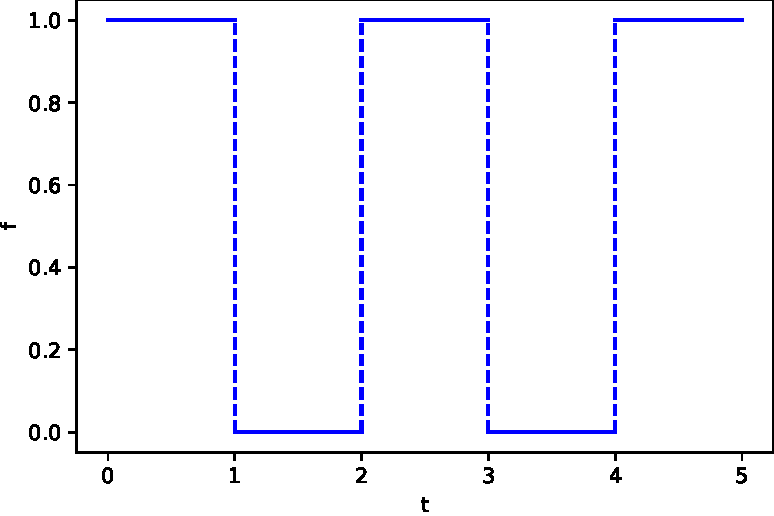
\includegraphics[width=0.6\textwidth]{DiscontEg.pdf}
		\caption{The discontinuous function $f(t)$ from \Cref{eg:disconteg}.}
		\label{fig:disconteg}
	\end{figure}
	
	We can write $f(t)$ in terms of step functions:
	\[
	f(t) = u_0(t) - u_1(t) + u_2(t) - u_3(t) + u_4(t) - u_5(t).
	\]
	Applying the Laplace transform to $f(t)$ yields
	\[
	F(s) = \frac{1-e^{-s}+e^{-2s}-e^{-3s}+e^{-4s}-e^{-5s}}{s}.
	\]
	Now we apply the Laplace transform to the entire ODE:
	\begin{align*}
		s^2Y(s) - 3sY(s) + 2Y(s) &= F(s) \\
		Y(s) = \frac{F(s)}{s^2-3s+2} &= \frac{1-e^{-s}+e^{-2s}-e^{-3s}+e^{-4s}-e^{-5s}}{s(s-1)(s-2)} \\
		&= G(s)(1-e^{-s}+e^{-2s}-e^{-3s}+e^{-4s}-e^{-5s}),
	\end{align*}
	where
	\[
	G(s) = \frac{1}{s(s-1)(s-2)} = \frac{A}{s} + \frac{B}{s-1} + \frac{C}{s-2} = \frac12\frac{1}{s} - \frac{1}{s-1} + \frac12\frac{1}{(s-2)}.
	\]
	Applying the inverse Laplace transform to $G(s)$ gives
	\[
	g(t) = \frac12\left(1 - 2e^t + e^{2t}\right),
	\]
	so by applying the property in \Cref{eq:laplacediscont}, we find the solution to be
	\[
	y(t) = g(t) - g(t-1)u_1(t) + g(t-2)u_2(t) - \cdots - g(t-5)u_5(t).
	\]
\end{eg}

\begin{eg}
	Solve the initial value problem
	\begin{align*}
		2y'' + y' + 2y &= u_5(t) - u_{20}(t) = \begin{cases}
			1, & 5 \leq t < 20 \\
			0, & 0 \leq t < 5 \text{ and } t \geq 20
		\end{cases} \\
		y(0) &+ y'(0) = 0.
	\end{align*}
	First, take the Laplace transform:
	\begin{align*}
		2s^2Y - 2sy(0) - 2y'(0) + sY - y(0) + 2Y &= \frac{e^{-5s} - e^{-20s}}{s} \\
		Y(s) &= \frac{e^{-5s} - e^{-20s}}{s(2s^2 + s + 2)} \\
		&= (e^{-5s} - e^{-20s})G(s),
	\end{align*}
	where
	\[
		G(s) = \frac{1}{s(2s^2 + s + 2)}.
	\]
	Recall the t-shift: $e^{-sc}G(s) = \Lap{g(t-c)u_c(t)}(s)$. Therefore
	\[
		y(t) = u_5(t)g(t-5) - u_{20}(t)g(t-20), \quad\text{with}\quad g(t) = \Lapinv{G(s)}.
	\]
	Now we decompose $G(s)$ into partial fractions:
	\[
		G(s) = \frac{a}{s} + \frac{bs+c}{2s^2+s+2} = \frac{1/2}{s} - \frac{s+1/2}{2s^2+s+2}.
	\]
	To deal with the second term, complete the square in the denominator:
	\[
		\frac{s+\sfrac12}{2s^2+s+2} = \frac12 \frac{(s+\sfrac14)+\sfrac14}{(s+\sfrac14)^2+\sfrac{15}{16}}.
	\]
	Using the results (see \Cref{table:laplace})
	\[
		\Lap{e^{at}\sin(bt)} = \frac{b}{(s-a)^2+b^2}, \quad \Lap{e^{at}\cos(bt)} = \frac{s-a}{(s-a)^2+b^2}
	\]
	we derive
	\[
		g(t) = \frac12 - \frac12 \left(e^{-t/4}\cos\left(\frac{\sqrt{15}}{4}t\right) + \frac{1}{\sqrt{15}} e^{-t/4}\sin\left(\frac{\sqrt{15}}{4}t\right)\right).
	\]
	Therefore the solution for $y(t)$ is
	\[
		y(t) = u_5(t)g(t-5) - u_{20}g(t-20)
	\]
	where $g(t)$ is given above.
\end{eg}

\subsection{Solving ODEs with Impulsive Forcing}

Impulsive forcing in an ODE $ay''+by'+cy=g(t)$ means that the inhomogeneity $g(t)$ acts only for a short period of time, $t_0\tau < t < t_0+\tau$.

With such an ODE, we want to impose the condition on the impulse
\[
	I(\tau) = \int_{t_0-\tau}^{t_0+\tau} g(t) \,dt = 1.
\]
This impulse provides a measure of the strength of the forcing term $g(t)$. The intuitive idea is that we are considering a forcing that is very short in duration, but large enough in magnitude that it has a significant effect on $y(t)$, for example a hammer blow in a mechanical system.

Taking $t_0$ for convenience, there are a few different options for modelling the impulse $g(t)$. They are listed below, and shown in \Cref{fig:impulsivefuncs}.
\begin{itemize}
	\item Top hat function: $g(t) = \begin{cases}\frac{1}{2\tau} & \text{if }-\tau \leq t \leq \tau \\ 0 & \text{otherwise}\end{cases}$.
	\item $g(t) = \dfrac{\tau}{\pi(t^2+\tau^2)}$
	\item Gaussian: $g(t) = \dfrac{1}{\sqrt{2\pi\tau^2}}e^{-t^2/2\tau^2}$.
\end{itemize}

\begin{figure}[!ht]
	\centering
	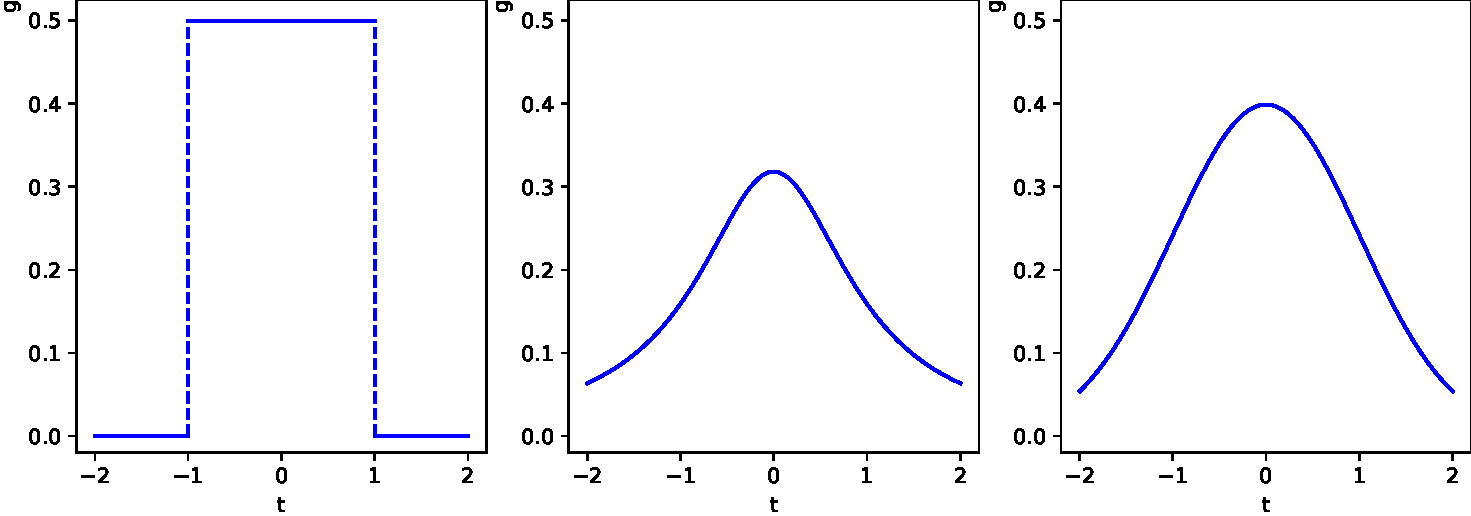
\includegraphics[width=0.9\textwidth]{ImpulsiveFunctions.pdf}
	\caption{The three examples of functions $g(t)$ for modelling impulses, setting $\tau=1$, in the order in the list from left to right.}
	\label{fig:impulsivefuncs}
\end{figure}

As $\tau \to 0$, these functions all converge to the same function: the \textbf{Dirac distribution}.

\begin{definition}
	The Dirac distribution is a ``function'' $\delta(t)$ such that
	\begin{itemize}
		\item $\delta(t)=0$ for all $t \neq 0$,
		\item $\int_{-\infty}^{\infty} \delta(t)\,dt = 1$.
	\end{itemize}
\end{definition}

With the shifted version of the Dirac distribution, it is centred at $t-t_0$ and we have $\delta(t-t_0)=0, \,\, \forall t\neq t_0$, and $\int_{-\infty}^{\infty} \delta(t-t_0)\,dt = 1$.

A key property of the Dirac distribution is that
\[
\int_{-\infty}^{\infty} f(t)\delta(t-t_0)\,dt = f(t_0).
\]
Applying the Laplace transform to the Dirac distribution:
\begin{equation*}
	\Lap{\delta(t-t_0)} = \int_0^{\infty} e^{-st}\delta(t-t_0) \,dt = e^{-st_0}. \tag{$t_0>0$}
\end{equation*}
By convention, we say that
\[
\delta(t) = \lim_{t_0 \to 0^+}\delta(t-t_0) \implies \Lap{\delta(t)} = 1.
\]

\begin{remark}
	From \Cref{eq:laplacediscont} and setting $f(t)=1$,
	\[
	\Lap{u_{t_0}(t)} = \frac{e^{-st_0}}{s}.
	\]
	Therefore
	\[
	\Lap{\delta(t-t_0)} = e^{-st_0} = s\Lap{u_{t_0}(t)} = \Lapb{\frac{d}{dt}u_{t_0}(t)}.
	\]
	Which implies that
	\[
	\text{$\delta(t-t_0)$ ``='' $\frac{d}{dt}u_{t_0}(t).$}
	\]
\end{remark}

We can do a check that $\Lap{\delta(t-t_0)} = e^{-st_0}$ makes sense by considering $\delta(t-t_0)$ as the limit as $\tau\to0$ of the top hat function in \Cref{fig:impulsivefuncs}:
\begin{align*}
	\delta(t-t_0) &= \lim_{\tau\to0} (\text{top hat function}) \\
	&= \lim_{\tau\to0} \frac{1}{2\tau}\left(u_{t_0-\tau}(t) - u_{t_0+\tau}(t)\right) = \lim_{\tau\to0} g(t,t_0).
\end{align*}
Then calculating $\Lap{g(t,t_0)}$:
\begin{align*}
	\Lap{g(t,t_0)} &= \frac{1}{2\tau} \left(\frac{e^{-s(t_0-\tau)}}{s} - \frac{e^{-s(t_0+\tau)}}{s}\right) \\
	&= \frac{e^{-st_0}}{2\tau s} (e^{s\tau}-e^{-s\tau}) \\
	&= e^{-st_0} \frac{\sinh(s\tau)}{s\tau}.
\end{align*}
Since $\lim_{x\to0} \frac{\sinh(x)}{x} = 1$, we have that
\[
\lim_{\tau\to0} \Lap{g} = e^{-st_0} = \Lap{\delta(t-t_0)}.
\]

As another check, consider the following initial value problem:
\[
y''+y = f_a(t) = \frac{1}{a}\left(u_0(t)-u_a(t)\right), \quad\text{with}\quad y(0)=y'(0)=0,
\]
where $f_a(t)$ is shown in \Cref{fig:impulseeg}.

\begin{figure}[H]
	\centering
	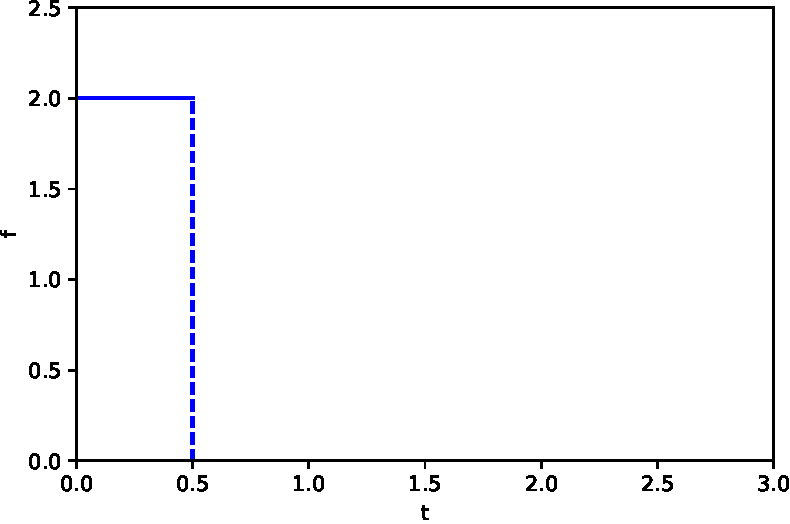
\includegraphics[width=0.5\textwidth]{ImpulseEg.pdf}
	\caption{The function $f_a(t)$ used in the check, taking $a=\frac12$.}
	\label{fig:impulseeg}
\end{figure}

Applying the Laplace transform to both sides:
\begin{align*}
	s^2Y + Y &= \frac{1}{a}\left(\frac{1}{s} - \frac{e^{-as}}{s}\right) \\
	Y(s) &= \frac{1-e^{-as}}{as(s^2+1)} = G(s)(1-e^{-as}),
\end{align*}
where
\begin{align*}
	G(s) &= \frac{1}{as(s^2+1)} = \frac{1}{a} \left(\frac{1}{s} - \frac{s}{s^2+1}\right) \\
	\implies g(t) &= \frac{1}{a} \left(u_0(t) - \cos(t)u_0(t)\right).
\end{align*}
Note that the $u_0(t)$ terms are introduced to ensure that $g(t)$ (and therefore $y(t)$) is zero for $t<0$. Therefore
\begin{align*}
	y(t) &= \frac{1}{a} \left(u_0(t)(1-\cos(t)) - u_a(t)(1-\cos(t-a))\right) \\
	&= \begin{cases}0 & \text{if }t<0 \\ \frac{1}{a}(1-\cos(t)) & \text{if } 0 \leq t \leq a \\ \frac{1}{a}(\cos(t-a)-\cos(t)) & \text{if } t>a \end{cases}.
\end{align*}
Taking the limit as $a \to 0$
\[
\frac{1}{a}(\cos(t-a)-\cos(t)) = \frac{1}{a}(\cos{t}\cos{a} + \sin{t}\sin{a} - \cos{t}) \to \sin{t}
\]
Therefore
\[
y(t) = \begin{cases}0 & \text{if } t<0 \\ \sin{t} & \text{if } t>a>0 \end{cases}.
\]

This is what we find by first solving the differential equation then taking the limit of this solution as $a \to 0$. Now we do this the other way around: taking the limit then solving:
\begin{align*}
	y'' + y &= \delta(t) \\
	s^2Y + Y &= 1 \\
	Y(s) &= \frac{1}{s^2+1} \\
	\implies y(t) &= \sin{t}.
\end{align*}
This is of course the same result - this direction of calculation is much faster and more convenient.

\begin{eg}
	We solve the ODE
	\[
	2y''+y'+2y=\delta(t-5) \quad\text{with}\quad y(0)=y'(0)=0.
	\]
	Applying the Laplace transform:
	\[
	2s^2Y + sY + 2Y = e^{-5s}.
	\]
	Therefore
	\begin{align*}
		Y(s) &= \frac{e^{-5s}}{2s^2+s+2} = \frac12 \frac{e^{-5s}}{(s+\sfrac14)^2+\sfrac{15}{16}} \\
		&= \frac12 e^{-5s} \frac{4}{\sqrt{15}} \frac{\sqrt{15}/4}{(s+\sfrac14)^2+\sfrac{15}{16}}.
	\end{align*}
	Recognising that the final fraction is the Laplace transform of $e^{-t/4}\sin\left(\frac{\sqrt{15}}{4}t\right)$ (see \Cref{table:laplace}) we invert the transform (also dealing with the $e^{-5s}$ by inverting an s-shift) and find that
	\begin{align*}
		y(t) &= \frac12 \frac{4}{\sqrt{15}} e^{-(t-5)/4} \sin\left(\frac{\sqrt{15}}{4}(t-5)\right) u_5(t) \\
		&= \frac{2}{\sqrt{15}} e^{-(t-5)/4} \sin\left(\frac{\sqrt{15}}{4}(t-5)\right) u_5(t)
	\end{align*}
\end{eg}


\subsection{Convolution of Two Functions}

The convolution of two functions $f(t)$ and $g(t)$ is given by:
\begin{equation}
	(f * g)(t) = \int_0^t f(\tau)g(t - \tau) \,d\tau = \int_0^t f(t - \tau)g(\tau) \,d\tau.
\end{equation}

Properties of Convolution:
\begin{enumerate}
	\item Distributive: $f*(g+h) = (f*g)+(f*h)$.
	\item Commutative: $f*g = g*f$.
	\item Associative: $f*(g*h) = (f*g)*h$.
\end{enumerate}

\begin{proof}\hfill
	\begin{enumerate}
		\item The distributive property follows easily from the definition and linearity of the integral.
		\item To prove the commutative property, begin with the definition of the convolution:
		\[
		(f*g)(t) = \int_0^t f(\tau) g(t-\tau) \,d\tau.
		\]
		We make a change of variables $\tau' = t - \tau$. Changing the constants of integration,
		\[
		(f*g)(t) = \int_0^t f(t - \tau') g(\tau) \,d\tau' = (g*f)(t)
		\]
		\item To prove the associative property:
		\begin{align*}
			f*(g*h) & = \int_0^t f(\tau) \,d\tau \int_0^{t-\tau '} h(\tau') g(t - \tau - \tau ') \,d\tau' \\
			& = \int_0^{t} h(\tau')\,d\tau' \int_0^{t-\tau'} f(\tau) g(t - \tau - \tau ') \,d\tau \\
			& = h*(f*g) = (f*g)*h,
		\end{align*}
		where $h*(f*g) = (f*g)*h$ follows since we have already proved commutativity.
	\end{enumerate}
\end{proof}

\subsubsection{Convolution Theorem}

\begin{theorem}[Convolution theorem]
	If $F(s) = \Lap{f(t)}$ and $G(s) = \Lap{g(t)}$ both exist for $s > a \geq 0$, then
	\[
	H(s) = F(s)G(s) = \Lap{f*g}.
	\]
	In other words, the Laplace transform of the convolution is the product of the Laplace transforms for the individual functions.
\end{theorem}

\begin{proof}
	From the definition of the convolution and Laplace transform, we have
	\begin{align*}
		\Lap{(f*g)}(s) &= \int_0^{\infty} e^{-st}\,dt \int_0^t f(\tau)g(t-\tau)\,d\tau.
		\intertext{By changing the ranges of integration:}
		&= \int_0^{\infty} f(\tau) \,d\tau \int_{\tau}^{\infty} e^{-st} g(t-\tau) \,dt 
		\intertext{Making a change of variables $t-\tau = \tau'$:}
		&= \int_0^{\infty} f(\tau) \,d\tau \int_0^{\infty} e^{-s(\tau' + \tau)}g(\tau') \,d\tau' \\
		&= \int_0^{\infty} f(\tau)e^{-s\tau}\,d\tau \int_0^{\infty} e^{-s\tau'}g(\tau')\,d\tau'\\
		&= \Lap{f} \Lap{g}
	\end{align*}
\end{proof}

This theorem is useful for inverting Laplace transforms, since
\[
\Lapinv{F(s)G(s)} = (f*g)(t).
\]

\subsubsection{Application to Second-Order ODEs}

\begin{eg}
	We solve the ODE
	\[
	y'' + \omega^2y = f(t) \quad\text{with}\quad y(0) = y'(0) = 0.
	\]
	Applying the Laplace transform to both sides of the equation,
	\begin{align*}
		s^2Y(s) + \omega^2Y(s) = F(s) = \Lap{f}(s) \\
		Y(s) = \frac{F(s)}{s^2+\omega^2} = F(s) \frac{1}{s^2 + \omega^2}.
	\end{align*}
	If we apply the inverse Laplace transform to:
	\begin{itemize}
		\item From $F(s)$, we get $f(t)$. 
		\item From $\frac{1}{s^2+\omega^2}$, we get $\frac{1}{\omega} \sin(\omega t)$.
	\end{itemize}
	So
	\[
	y(t) = \frac{1}{\omega} \int_0^t f(\tau)\sin\left(\omega(t-\tau)\right) \,d\tau.
	\]
\end{eg}

We can also use the Convolution theorem to find a general procedure for solving second-order ODEs. Consider the second-order ODE
\[
	ay'' + by' + cy = f(t) \quad\text{with}\quad y(0) = y_0, \,\, y'(0) = y_0'.
\]
Applying the Laplace transform, we have
\begin{align*}
	a(s^2Y - sy_0 - y_0') + b(sY-y_0)+cY &= F(s) \\
	\implies (as^2+bs+c)Y(s) &= F(s) + (as+b)y_0 + ay_0' \\
	\implies Y(s) &= \frac{1}{as^2+bs+c} \left(F(s) + G(s)\right) \\
	\implies Y(s) &= H(s)\left(F(s)+G(s)\right),
\end{align*}
where $H(s) = \frac{1}{as^2+bs+c}$, and $G(s) = (as+b)y_0 + ay_0'$.

Okay, so let's take a trip to the Laplace world now! For $Y$, the response to forcing and to initial conditions is split into 2 parts:
\begin{itemize}
	\item $F(s)$ is a response from forcing.
	\item $G(s)$ is a response that depends on the initial conditions. 
	\item $H(s)$ helps transfer these into the solution $Y$ so (surprise surprise!) $H(s)$ is called a transfer function.
\end{itemize}

By the convolution theorem, if we have the inverse Laplace transforms of $F$, $G$, and $H$ then we can find the solution $y(t)$ as:
\[
y(t) = \int_0^t h(t-\tau)f(\tau) \,d\tau + \int_0^t h(t-\tau)g(\tau)\,d\tau.
\]

\underline{Transfer Function}:
\[
H(s) = \frac{1}{as^2+bs+c}
\]
has a Laplace inverse given by $\Lapinv{H} = h(t)$, where 
\[
ah'' + bh' + ch = \delta(t), \quad\text{with}\quad h(0) = h'(0) = 0,
\]
where $\delta(t)$ is a Dirac distribution. So $h(t)$ is a solution to a differential equation where the forcing is just a distribution.

Thus, you can write the solution to any differential equation with constant coefficients as the sum of two convolutions, one relating to the forcing function $f(t)$, and the other relating to the initial conditions.

\begin{eg}
	We solve the ODE
	\[
	y''+4y = f(t) \quad\text{with}\quad y(0) = 3, \,\, y'(0) = 1.
	\]
	Applying the Laplace transform:
	\begin{align*}
		s^2Y - 3s - 1 + 4Y &= F(s) \\
		\implies (s^2+4)Y &= F(s)+3s+1 \\
		\implies Y(s) &= H(s) \left[ F(s) + 3s+1\right] \quad \text{where } H(s) = \frac{1}{s^2+4}.
	\end{align*}
	Applying the inverse Laplace transform to $H(s)$:
	\[
	h(t) = \frac12 \sin{2t}.
	\]
	Therefore
	\begin{align*}
		Y(s) &= H(s)F(s) + \frac{3s}{s^2+4} + \frac{1}{s^2+4} \\
		\implies y(t) &= \frac12 \int_0^t \sin\left(2(t-\tau)\right) f(\tau) \,d\tau + 3\cos{2t} + \frac12\sin{2t}.
	\end{align*}
\end{eg}

\subsubsection{Integral Equations}

We can use convolutions to solve integral equations; that is, equations in which a function $y(t)$ appears inside an integral. This is best illustrated by an example.

\begin{eg}
	We solve the integral equation
	\[
	y(t) = \int_0^t \cos{(t-\tau)}y(\tau)\,d\tau + 1.
	\]
	The RHS of the above equation is a convolution, so take Laplace transform on both sides 
	\begin{align*}
		Y(s) &= \frac{s}{s^2+1}Y(s) + \frac1s \\
		\implies \frac{s^2-s+1}{s^2+1}Y(s) &= \frac1s \\
		\implies Y(s) &= \frac{1+s^2}{s(s^2-s+1)} = \frac{s^2-s+1}{s(s^2-s+1)} + \frac{s}{s(s^2-s+1)} \\
		&= \frac1s + \frac{1}{s^2-s+1} = \frac1s + \frac{\sqrt{3}/2}{\left(s-1/2\right)^2 + 3/4} \cdot \frac{2}{\sqrt{3}}.
	\end{align*}
	Finally, we take the inverse Laplace transform of each of these terms:
	\[
	y(t) = 1 + \frac{2}{\sqrt{3}}e^{-t/2} \sin{\left(\frac{\sqrt{3}t}{2}\right)}.
	\]
\end{eg}

\begin{eg}
	Show that
	\[
		\phi(t) = \int_0^t \int_0^{t_1} \cdots \int_0^{t_{n-1}} f(t) dt_1 dt_2 \cdots dt_n = \int_0^t \frac{(t-\tau)^{n-1}}{(n-1)!} f(\tau)\,d\tau.
	\]
	First, notice that
	\[
		\Lapb{\int_0^t f(\tau)\,d\tau} = \Lapb{\int_0^t f(\tau) u_0(t-\tau) \,d\tau} =  \Lap{f*u_0} = \Lap{f}\Lap{u_0} = \frac{F(s)}{s}.
	\]
	Applying this property recursively, we find that
	\[
		\Lap{\phi} = \frac{F(s)}{s^n}.
	\]
	Then
	\[
		\Lapinvb{\frac{1}{s^n}} = \frac{t^{n-1}}{(n-1)!} \quad\text{since}\quad \Lap{t^n} = \frac{n!}{s^{n+1}}.
	\]
	Therefore, by the Convolution theorem,
	\[
		\Lap{\phi} = \Lapb{\frac{t^{n-1}}{(n-1)!}}\Lap{f(t)} = \Lapb{\int_0^t \frac{(t-\tau)^{n-1}}{(n-1)!} f(\tau)\,d\tau},
	\]
	and taking the inverse Laplace transform yields
	\[
		\phi(t) = \int_0^t \frac{(t-\tau)^{n-1}}{(n-1)!} f(\tau)\,d\tau.
	\]
\end{eg}

The Laplace transform can also be used to solve linear systems of ODEs.

\begin{eg}
	Solve the system of initial value problems
	\begin{align*}
		x'(t) - 2y(t) &= 4t, \quad x(0)=4 \\
		y'(t) + 2y(t) - 4x(t) &= -4t-2, \quad y(0)=-5
	\end{align*}
	Taking the Laplace transforms of both ODEs yields
	\begin{align*}
		sX(x) - 4 - 2Y(s) &= \frac{4}{s^2} \\
		sY(s) + 5 + 2Y(s) - 4X(s) &= -\frac{4}{s^2} - \frac{2}{s},
	\end{align*}
	where $X(s) = \Lap{x(t)}$ and $Y(s) = \Lap{y(t)}$.
	
	Solving the pair of transformed ODEs for $X(s)$, we find
	\[
		(s(s+2)-8)X(s) = \frac{(s+2)(4s^2+4)}{s^2} - \frac{10s^2+4s+8}{s^2},
	\]
	which simplifies to
	\[
		X(s) = \frac{4s-2}{(s+4)(s+2)} = \frac{3}{s+4} + \frac{1}{s-2}.
	\]
	Applying the inverse Laplace transform yields
	\[
		x(t) = 3e^{-4t} + e^{2t}.
	\]
	Then, rearranging the first ODE yields
	\[
		y(t) = \frac12 x'(t) - 2t = -6e^{-4t} + e^{2t} - 2t.
	\]
\end{eg}

\begin{exercise}
	The system of initial value problems in the above example can be written in matrix form as
	\[
		\xtp = \mat{0 & 2 \\ 4 & -2}\xt + \mat{4t \\ -4t - 2}, \quad \vbx(0) = \mat{4 \\ -5}.
	\]
	Using the methods of \Cref{sec:firstorder}, solve this system and confirm that the result is equivalent to the solution obtained using the Laplace transform.
\end{exercise}

\pagebreak
\subsection{Table of Elementary Transforms}\label{sec:laptable}

\begin{table}[!ht]
	\begin{center}
		\begin{tabular}{>{$}c<{$}|>{$}c<{$}}
			f(t) = \Lapinv{F(s)} & F(s) = \Lap{f(t)} \\
			\hline
			1 & \dfrac{1}{s}, \quad s>0 \rule{0pt}{1.8em}\\[1em]
			e^{at} & \dfrac{1}{s-a}, \quad s>0 \\[1em]
			t^n, \quad n \in \mathbb{N} & \dfrac{n!}{s^{n+1}}, \quad s>0 \\[1em]
			t^p, \quad p>-1 & \dfrac{\Gamma(p+1)}{s^{p+1}}, \quad s>0 \\[1em]
			\sin(at) & \dfrac{a}{s^2+a^2}, \quad s>0 \\[1em]
			\cos(at) & \dfrac{s}{s^2+a^2}, \quad s>0 \\[1em]
			\sinh(at) & \dfrac{a}{s^2-a^2} \quad s>|a| \\[1em]
			\cosh(at) & \dfrac{s}{s^2-a^2} \quad s>|a| \\[1em]
			e^{at}\sin(bt) & \dfrac{b}{(s-a)^2+b^2}, \quad s>a \\[1em]
			e^{at}\cos(bt) & \dfrac{s-a}{(s-a)^2+b^2}, \quad s>a \\[1em]
			t^ne^{at}, \quad n\in\mathbb{N} & \dfrac{n!}{(s-a)^{n+1}}, \quad s>a \\[1em]
			u_c(t) = \begin{cases}0 & t<c \\ 1 & t\geq c\end{cases} & \dfrac{e^{-cs}}{s}, \quad s>0 \\[1em]
			u_c(t)f(t-c) & e^{-cs}F(s) \\[1em]
			e^{-ct}f(t) & F(s+c) \\[1em]
			tf(t) & -\dfrac{d}{ds}F(s) \\[1em]
			(-t)^nf(t) & F^{(n)}(s) \\[1em]
			f(ct) & \dfrac{1}{c}F\left(\dfrac{s}{c}\right), \quad c>0 \\[1em]
			\delta(t-c) & e^{-cs} \\[1em]
			\delta(t-c)f(t) & e^{-cs}f(c) \\[1em]
			f^{(n)}(t) & s^nF(s) - s^{n-1}f(0) - \cdots - f^{(n-1)}(0) \\[1em]
			(f*g)(t) = \int_0^t f(\tau)g(t-\tau)\,d\tau & F(s)G(s)
		\end{tabular}
	\end{center}
	\caption{Elementary Laplace Transforms.}
	\label{table:laplace}
\end{table}